\subsection{Spændingsforsyning}
Spændingsforsyningen skal være i stand til at forsyne kredsløbets aktive komponenter med en konstant spænding. Den anvendte spændingsforsyning er en færdigudviklet komponent, som består af to batterier på $1,5~V$, der sidder i en spændingsregulator. Batteriernes kobling danner et split supply, og derfor dannes der en jordforbindelse fra det ene batteris negative pol og den andens positive pol. De andre poler, som ikke anvendes til jordforbindelse, benyttes som systemets positive spændingsforsyning, ${V}_{cc}$ og negative spændingsforsyning, ${V}_{dd}$.
Spændingsregulatoren sørger for at give en jævn spænding på henholdsvis $3,4~V$ og $\pm 5,5~V$. Dette gøres ved, at spændingsregulatoren oplagre spænding fra de to tilkoblede batterier i spoler, når switchfunktionen lukkes. Switchfunktionen åbnes når spolerne er mættet og en spænding ledes videre i kredsløbet via en diode. Denne switchfunktion åbner og lukker skiftevis i kort tid, hvilket gør, at der hele tiden ledes en konstant spænding til systemet. Da batterierne med tiden vil løbe tør for spænding, vil der ikke leveres en jævnspænding, hvor ved systemet ikke vil fungere optimalt. For at undgå dette gør spændingsregulatoren opmærksom på dette ved at få en LED til at blinke når den ikke leverer en konstant spænding. 
Konfigurationen af spændingsforsyningen fremgår af \autoref{fig:spaendingsforsyning}, hvor terminalerne for $\pm 5,5~V$ fremgår som rød(V+) og blå(V-) og sort(Gnd), mens der på den modsatte side fremgår terminalerne for $3,4~V$ som brun(Vcc) og sort(Gnd). 

\begin{figure}[H]
\centering
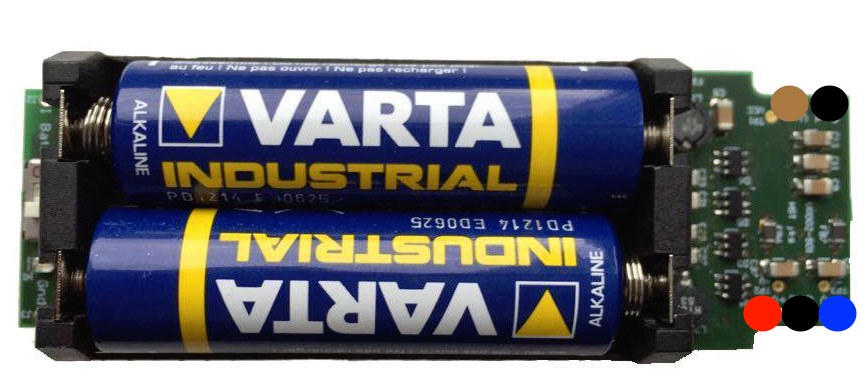
\includegraphics[width=0.5\textwidth]{figures/spaendingsforsyning}
\caption{Spændingsforsyning, der består af to $1,5~V$ batterier i et split supply. Den røde prik illustrerer V+, den blå V-, den sorte Gnd og den brune Vcc.}
\label{fig:spaendingsforsyning}
\end{figure}

%\vspace{3mm}
\textbf{Krav:}
\begin{itemize} 
\item Skal kunne forsyne aktive komponenter i den analoge del af kredsløbet
\item Skal få en LED til at lyse hvis den ikke levere en konstant spænding
%\item Skal forsyne mikrokontrolleren
%\item Skal være batteridrevet 
\end{itemize}
